% Chapter 7
\chapter{The Search for the Cause of the Gap}
\label{ch:gap}

This chapter addresses RQ2. It tests the possible causes of the gap one at a time. \Cref{fig:timeline} shows the order of the work.

\begin{figure}[ht]
\centering
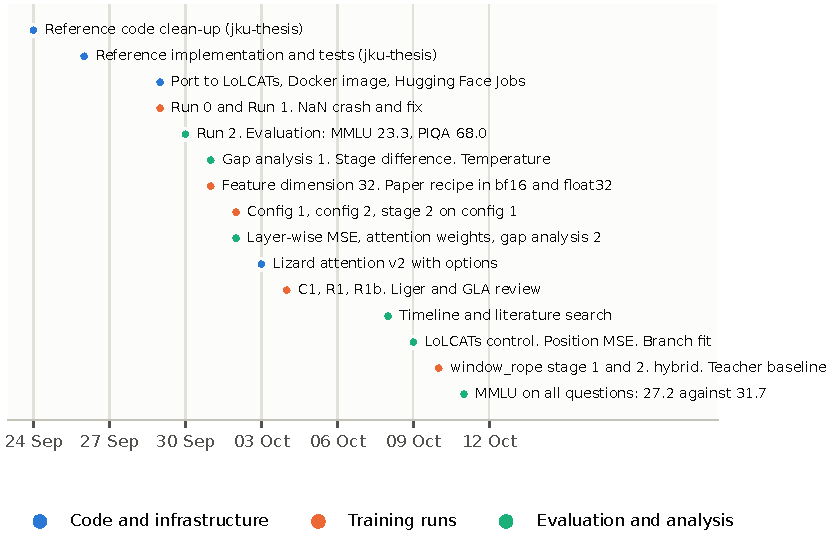
\includegraphics[width=\linewidth]{timeline}
\caption[Timeline of the project]{Timeline of the project, from the pull requests of the two repositories and the project notes (document~18).}
\label{fig:timeline}
\end{figure}

\section{The possible causes}
\label{sec:causes}

The tests of \cref{sec:tests} excluded a bug in the formulas. The first gap analysis ranked the remaining causes (\cref{tab:causes}). The recipe had the largest difference from the paper, so it came first. A missing checkpoint key was cheap to check, so it came next.

\begin{table}[ht]
\centering
\small
\caption[Ranking of the possible causes after the first reproduction]{Ranking of the possible causes after the first reproduction (project notes, document~11), and the later result of each test.}
\label{tab:causes}
\begin{tabularx}{\linewidth}{@{}rLL@{}}
\toprule
\# & Possible cause & Result of the test \\
\midrule
1 & The stage 1 recipe differs from the paper & Not the main cause (\cref{sec:recipe-exp}) \\
2 & The stage 2 recipe and the frozen Lizard parameters & No change in accuracy (\cref{sec:stage2-paper}) \\
3 & Missing keys when the checkpoint loads & Excluded: 0 missing keys in every evaluation \\
4 & The data, the packing or the prompts & Not tested. The data and the packing follow the paper. \\
5 & Numerical effects of bf16 & Real for the recipe of the paper (\cref{sec:precision}) \\
6 & The harness version & Small: the teacher gets the paper values (\cref{tab:teacher}) \\
7 & The tokenization of the MMLU letters & Excluded: each letter is one token \\
8 & The checkpoint selection & Excluded: the best step is the last evaluation in all runs but one \\
9 & The version of the \code{transformers} library & Not tested \\
\bottomrule
\end{tabularx}
\end{table}

\section{Precision: bf16 can discard small updates}
\label{sec:precision}

The first runs store the model and the trainable weights in bf16. This format keeps only approximately 3 significant digits. An AdamW step changes a weight by approximately the learning rate. If the step is smaller than half the distance between two neighboring bf16 numbers, rounding discards it. At the stage 1 learning rate of LoLCATs ($10^{-2}$), rounding discards no updates. At the stage 2 learning rate ($10^{-4}$), it discards 43--65\% of the LoRA updates. At $10^{-3}$, the learning rate of the paper, it discards every update of $\alpha$, because $\alpha$ starts at 1.0.

A stage 1 run with the learning rate and the schedule of the paper showed this effect. In bf16, $\alpha$ stayed at exactly 1.000 in all 16 layers. The validation loss was 8.1641, 2.4 times the loss of the LoLCATs recipe. The same recipe with all weights, the optimizer states and the target in float32 moved $\alpha$ to 0.60--0.79 and lowered the loss to 4.9478. All later runs with the recipe of the paper use float32.

\section{The recipe experiments}
\label{sec:recipe-exp}

Each experiment changed one part of the recipe. These runs use feature dimension 32, the LoLCATs rule for a head dimension of 64. A separate run showed that this value is not a cause. It gave a loss of 3.4219 against 3.2549 for 128, and the gate saturated in the same way. \Cref{tab:recipe-runs} gives the results.

\begin{table}[ht]
\centering
\small
\caption[Stage 1 runs with different recipes]{Stage 1 runs with different recipes (project notes, documents~12 and 14). All runs use the original Lizard attention. Accuracy in \% after stage 1. PIQA has an SE of approximately 1.2 points, and ARC-Easy approximately 1.0 point.}
\label{tab:recipe-runs}
\begin{tabularx}{\linewidth}{@{}Lrrrr@{}}
\toprule
Stage 1 run & Loss & MMLU subset & PIQA & ARC-Easy \\
\midrule
Feature dimension 128, LoLCATs recipe, bf16 (Run 1) & 3.2549 & 22.5 & 57.6 & 39.0 \\
Feature dimension 32, LoLCATs recipe, bf16 & 3.4219 & 23.2 & -- & -- \\
Recipe of the paper, bf16 & 8.1641 & 25.3 & 55.8 & 34.1 \\
Recipe of the paper, float32 & 4.9478 & 24.6 & 57.7 & 35.7 \\
Config 1: also $\beta_2 = 0.99$ and a minimum learning rate & 3.9764 & 26.7 & 57.3 & 36.5 \\
Config 2: config 1 with gradient clipping at 1.0 & 3.5092 & 23.2 & 57.5 & 35.6 \\
\bottomrule
\end{tabularx}
\end{table}

Each step toward the recipe of the paper lowered the loss. With all optimizer settings of Table~13, the recipe of the paper came near the LoLCATs recipe, but it did not pass it. The accuracies stayed in small ranges: 55.8--57.7 on PIQA and 34.1--36.5 on ARC-Easy. With unpaired SEs, none of these differences is clear.

One result was clear. The recipe of the paper stops the saturation of the gate. With the LoLCATs recipe, the gate stays above 0.999 for every token in 14 or 15 of the layers 1--15. With the recipe of the paper, no layer saturates fully. Thus the high learning rate of LoLCATs causes the saturation. But a gate that decays did not give a better model either.

\section{Stage 2 with the recipe of the paper}
\label{sec:stage2-paper}

Stage 2 on config 1 used the stage 2 settings of Table~13 (learning rate $5 \times 10^{-4}$, LoRA on $q$, $k$ and $v$) in float32. Its validation loss was 1.9158, 14.9\% lower than in Run~2 (2.252). But its scores were almost the same: PIQA 67.7 against 67.95, and ARC-Easy 54.9 against 54.8. On the MMLU subset, it gave \enquote{A} for 77.5\% of the questions. \Cref{fig:stage1to2} shows that both stage 2 recipes add approximately 10 points on PIQA and approximately 16--18 points on ARC-Easy. The stage 1 differences did not reach the final model. Stage 2 changed the memory of the gate: in layers 9--15, the weight kept after 512 tokens fell from 0.48--0.94 to below 0.003. The gate parameters stayed frozen. Thus LoRA changed the hidden states that the gate reads.

\begin{figure}[ht]
\centering
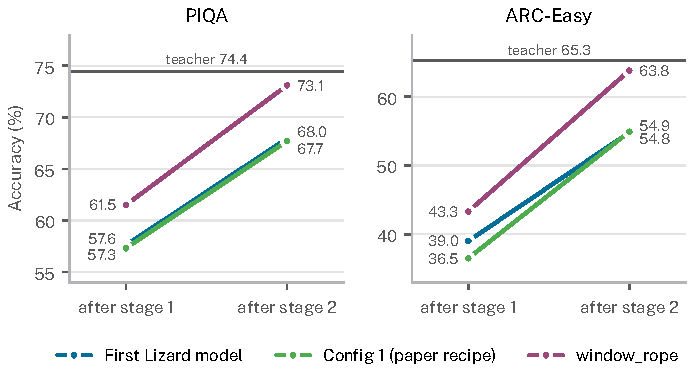
\includegraphics[width=\linewidth]{stage1_to_stage2}
\caption[PIQA and ARC-Easy after stage 1 and after stage 2]{PIQA and ARC-Easy after stage 1 and after stage 2, for three models. The first Lizard model and config 1 end at almost the same values. The \code{window_rope} model of \cref{ch:rope} starts higher and ends higher.}
\label{fig:stage1to2}
\end{figure}

\section{A lower loss does not give a higher accuracy}
\label{sec:loss-vs-acc}

Over the stage 1 runs, the loss fell from 8.16 to 3.05, but PIQA and ARC-Easy did not increase. Over the six runs with ARC-Easy, the rank correlation (Spearman) between the loss and the accuracy is +0.31 for ARC-Easy and $-0.06$ for PIQA. A positive value means that a lower loss comes with a lower accuracy. With six runs, none of these values is clear. \Cref{fig:loss-acc} shows all stage 1 runs of this thesis. Only the runs with RoPE in the window (orange) and the LoLCATs control (green) leave the cluster.

\begin{figure}[ht]
\centering
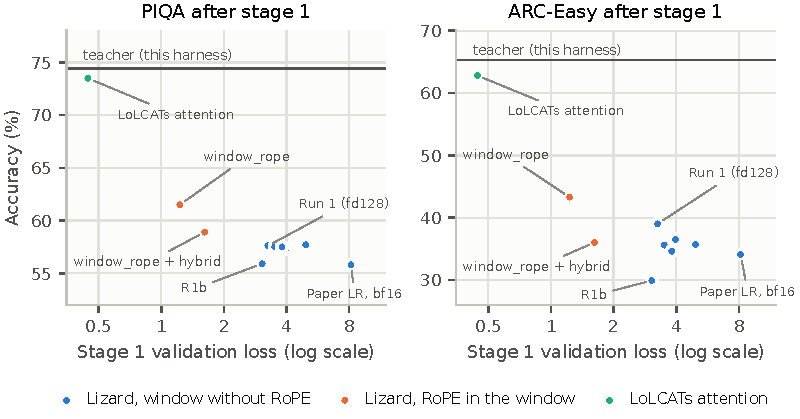
\includegraphics[width=\linewidth]{loss_vs_accuracy}
\caption[Stage 1 loss against the accuracy after stage 1]{Stage 1 loss against the accuracy after stage 1. Each point is one stage 1 run. The unlabeled blue points are the paper recipe in float32, config 1, config 2 and C1. Values in \cref{tab:recipe-runs,tab:v2-runs,tab:control} and Appendix~\ref{app:runs}.}
\label{fig:loss-acc}
\end{figure}

Three properties of the loss can explain this:
\begin{itemize}
\item The loss measures each layer alone, with the input of the teacher. It cannot see an error that grows from layer to layer.
\item All 2048 positions count the same. Positions 0--127 give only 6.25\% of the loss. But almost all PIQA and ARC-Easy prompts are shorter than 128 tokens.
\item Each run has one seed. Thus the noise of the loss and of the scores is not known.
\end{itemize}

\section{A limit for each head}
\label{sec:head-limit}

The second gap analysis looked at the attention weights (\cref{sec:xai-weights}) and found a limit in the architecture. A Lizard row is the gated branch, with weights that sum to 1, plus $\alpha$ times the window branch, with weights that sum to $\rho_i \le 1$. Thus the share of the exact window in a row has an upper limit:
\begin{equation}
\text{window share}_i = \frac{\alpha \rho_i}{1 + \alpha \rho_i} \le \frac{\alpha}{1 + \alpha} .
\label{eq:ceiling}
\end{equation}
All 32 heads of a layer share $\alpha$, the gate, the feature maps and the sink logits. Only $\vq$, $\vk$ and $\vv$ differ between the heads, and stage 1 does not train them. The measurements reach the limit. In layer 15, head 14 of config 1, $\alpha = 0.576$, so the limit is 0.365. The measured window share is 0.365. But the teacher puts 91.3\% of the weight of this head inside the window. In layer 0, the LoLCATs recipe trained $\alpha$ down to 0.063. Then no head of layer 0 can take more than 6\% from the window. But layer 0 has local heads, for example a head that attends to the previous token.

This limit explains several observations. Local teacher heads match worst. All heads of a layer get almost the same long-range share. The training lowers $\alpha$ for the majority of heads, which need far tokens, and the local heads lose. The gated branch cannot become local for one head only, because all heads share one gate. And without RoPE, neither branch knows the relative position of two tokens.

\section{Design options of v2: C1, \code{joint} and \code{hybrid}}
\label{sec:v2-runs}

The options of v2 (\cref{tab:v2-options}) attack the limit. \Cref{tab:v2-runs} gives three runs with the stage 1 recipe of config 1.

\begin{table}[ht]
\centering
\small
\caption[Stage 1 runs with options of Lizard v2]{Stage 1 runs with options of Lizard v2 (project notes, document~13). Accuracy in \% after stage 1.}
\label{tab:v2-runs}
\begin{tabularx}{\linewidth}{@{}Lrrrrr@{}}
\toprule
Run & Loss & PIQA & ARC-Easy & MMLU subset & \enquote{A} \\
\midrule
Config 1 (reference) & 3.9764 & 57.3 & 36.5 & 26.7 & 51.2\% \\
C1: one $\alpha$ for each head & 3.8092 & 57.5 & 34.6 & 23.9 & 64.9\% \\
R1: per-head $\alpha$ and maps, \code{joint} & stopped & -- & -- & -- & -- \\
R1b: per-head $\alpha$ and maps, \code{hybrid}, $\alpha$ start 0.1 & \textbf{3.0542} & 55.9 & \textbf{29.9} & 24.9 & 90.2\% \\
\bottomrule
\end{tabularx}
\end{table}

C1 lowered the loss by 4.2\%, but the accuracy did not change. R1 stopped at 19\% of the first epoch, because \code{joint} gives the gated branch almost no weight at the start values (\cref{tab:proofs}, P6). R1b gave the lowest loss of all Lizard runs at that time, 23.2\% below config 1. But ARC-Easy fell by 6.6 points ($z \approx -4.9$). In layer 15, the shared gate fell to 0.128. Heads 14 and 23 improved by 76--78\%, but 28 of the 32 heads got worse. A short gate gives position information, so it helps local heads. But one gate for all heads takes the long range from the other heads.

\section{The LoLCATs attention as a control}
\label{sec:control}

The control run used the same pipeline, data, recipe and harness, with the original LoLCATs attention in place of Lizard. Thus a clear difference must come from the attention layer. \Cref{tab:control} gives the result.

\begin{table}[ht]
\centering
\small
\caption[The LoLCATs control against Lizard after stage 1]{The LoLCATs control against Lizard after stage 1 (project notes, \enquote{LoLCATs control}). Both runs use the LoLCATs recipe.}
\label{tab:control}
\begin{tabular}{@{}lrrr@{}}
\toprule
Measure & Lizard, Run 1 & LoLCATs control & Difference \\
\midrule
Stage 1 loss & 3.2549 & \textbf{0.4442} & 7.3$\times$ lower \\
PIQA & 57.6 & \textbf{73.5} & +15.9 ($z \approx 10$) \\
ARC-Easy & 39.0 & \textbf{62.8} & +23.8 ($z \approx 17$) \\
MMLU subset & 22.5 & 26.0 & +3.5 ($z \approx 1.0$) \\
\enquote{A} on MMLU & 95.4\% & 19.3\% & -- \\
Probability mass of the four letters & 0.018 & 0.962 & -- \\
\bottomrule
\end{tabular}
\end{table}

After stage 1 alone, the LoLCATs control is above the final first Lizard model on PIQA (+5.5 points) and ARC-Easy (+8.0 points). Thus the pipeline can train a much better model, and the gap comes from the Lizard layer. On short prompts, the control computes almost exactly the teacher attention. Its window has RoPE and covers 128--255 tokens. Its linear part acts only on tokens farther back. Its layer-wise MSE is 3.7 to 36.9 times lower than that of Lizard in every layer. Layer 0 has the largest difference. There, the control gives its window 79\% of the weight on far queries, but Lizard turned its window almost off ($\alpha = 0.042$). MMLU stays near chance for the control too, but the control keeps the answer format: 96.2\% of its probability goes to the four letters.

\section{Summary}
\label{sec:gap-summary}

\begin{finding}
\textbf{RQ2.} The recipe and the precision matter, but they do not explain the gap. bf16 discards small updates and freezes $\alpha$ at the learning rate of the paper. Lower stage 1 losses did not give higher accuracies. The evidence excludes the checkpoint loading, the temperature, the feature dimension and the harness. The LoLCATs control in the same pipeline reaches 98.8\% of the teacher on PIQA after stage 1 alone. Thus the cause is in the Lizard attention. The most probable mechanism is a limit for each head. Its parts are the shared parameters, the gated branch with the weight 1, the ceiling $\alpha/(1+\alpha)$ and the window without RoPE.
\end{finding}
